% vim:set et sw=2 ts=4 tw=72:
\chapter{Design and Implementation}\label{chap:design_and_implementation}

A model is difficult to assess directly, instead it is possible to
convert the model into visualizations, which can be assessed as a proxy
to the effectiveness of the model. This chapter presents various
visualizations that take advantage of the \mt{} model, and a tool,
called \tool{}, that uses these visualizations.

\tool{} is web-based to enable ease of use, requiring nothing more than
a web-browser to access, otherwise users would need to install the
software and the database of repository data.

\tool{} is designed with two uses-cases in mind, though a user may
freely switch between the cases as they work. Both use-cases are
designed with maintainers in mind.

\begin{textbox}
  \textbf{Use-Case 1: top-to-bottom approach}

  These users are maintaining a portion of the kernel and would like to
  pick and entire merge, including all commits being merged, and merge
  it directly into their version of the kernel.

  These users do not have a specific commit in mind.
\end{textbox}

\begin{textbox}
  \textbf{Use-Case 2: bottom-to-top approach}

  These are maintainers that start with a given commit and would like to
  understand what other changes are being made to integrate this commit.
  This is done by understanding the merges that the commit passes
  through toward integration, and finding the commits that are necessary
  for the integration of a given commit.

  These users do have a specific commit in mind.
\end{textbox}

The tool uses full-text search to gather the repository events that the
user is interested in, two summarization views, and three visualizations
of the \mt{} for the repository events.

\section{Search}\label{sec:search}

\evan{Should I put this section in the implementation details?}

\tool{} provides a search engine for navigating within the kernel
repository, filtering the repository events that are not relevant. The
search engine takes a plain-text query from the user and returns the
results ordered by the relevancy to the query. Relevancy is computed by
weighted similarity, taking into account the contents of the commit log,
the author name, the filenames, the commit hash, the date the commit was
authored, and the date the commit was committed. More information about
the design of the search engine are available in
Section~\ref{sub:full_text_search}.

Before presenting the results, the repository events are grouped by
\mt{} root. Each group of events has the link to the root at the
top, followed by a table of the relevant commits and merges from that
tree, shown in Figure~\ref{fig:linvis_search_results}. The table of
results includes the relevancy rank assigned by the search engine,
commit preview, author, commit date, and the authored date. The
\mt{} groups are ordered by the mean of the relevancy scores.

\begin{figure}[htpb]
  \centering
  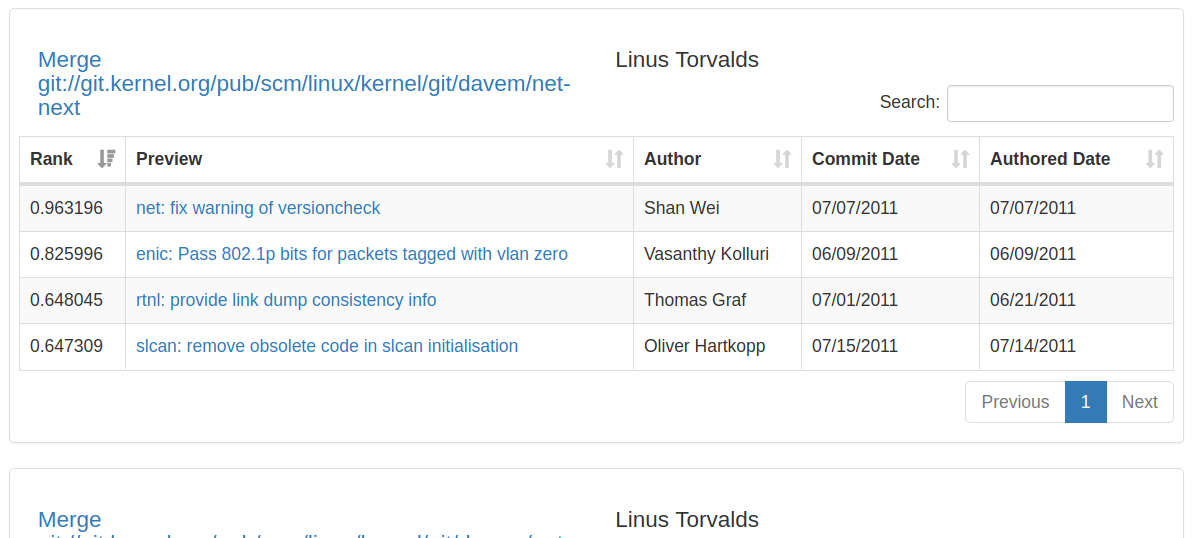
\includegraphics[width=0.9\linewidth]{Figures/Linvis/search_results.png}
  \caption{A single \mt{} in the search results of \tool{}, showing
    the link to the root at the top, and the relevant commits in the
    table below.}
  \label{fig:linvis_search_results}
\end{figure}

\section{Summarization}\label{sec:summarization}

\tool{} uses seven tabs to present the information and visualizations
for a selected repository event. The informative tabs are; messages,
files, modules, and authors. The visualization tabs are; list tree, pack
tree, and \rt{} tree.

The message tab shows the full commit log message. This does not include
the patch, but given a commit hash, the patch can be found directly from
the repository.

The files tab shows an aggregated table of all files that were modified
in a merge. It includes metrics like the number of lines added, lines
removed, total lines modified, and the delta, summed across all commits
in the \mt{} that modify the selected file. A details drop-down button
allows a user to see exactly which commits make the changes, as shown in
Figure~\ref{fig:linvis_files_results}.

\begin{figure}[htpb]
  \centering
  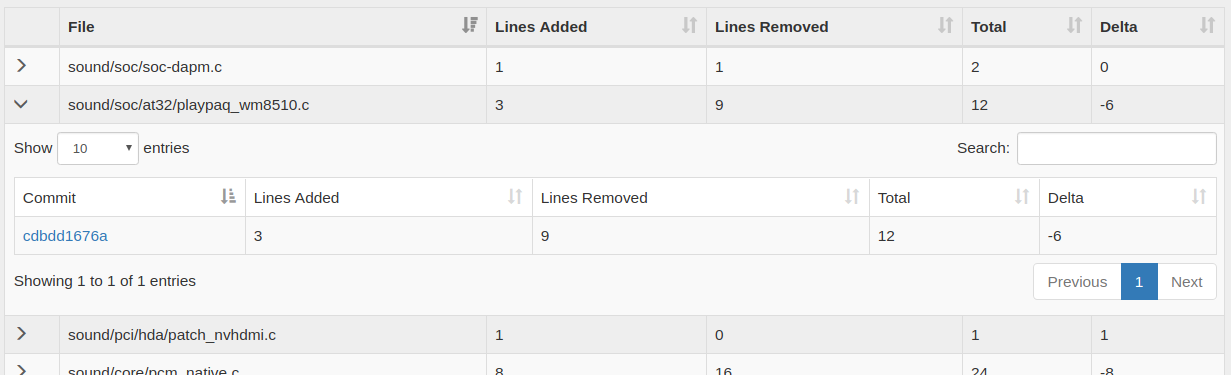
\includegraphics[width=0.9\linewidth]{Figures/Linvis/linvis_files.png}
  \caption{Table showing the modified files in a merge, with the second
    entry expanded to show the commit that makes the changes.}
  \label{fig:linvis_files_results}
\end{figure}

The modules tab shows the modules modified in the \mt{}. Like the files
tab, the modules tab uses a table to show the name of the module, the
number of commits that are in the \mt{} that work with the module, and a
details button to provide the links to those commits, shown in
Figure~\ref{fig:linvis_modules_results}. Modules are not an inherent
part of git, but are a property of most commit log previews in the Linux
repository. The text up to the first colon in the commit log preview
tends to indicate the subsystem of the kernel that is being modified. In
Figure~\ref{fig:sampleMerge}, the first commit is from the ``md''
subsystem, which virtualizes multiple physical devices into a single
virtual device.

\begin{figure}[htpb]
  \centering
  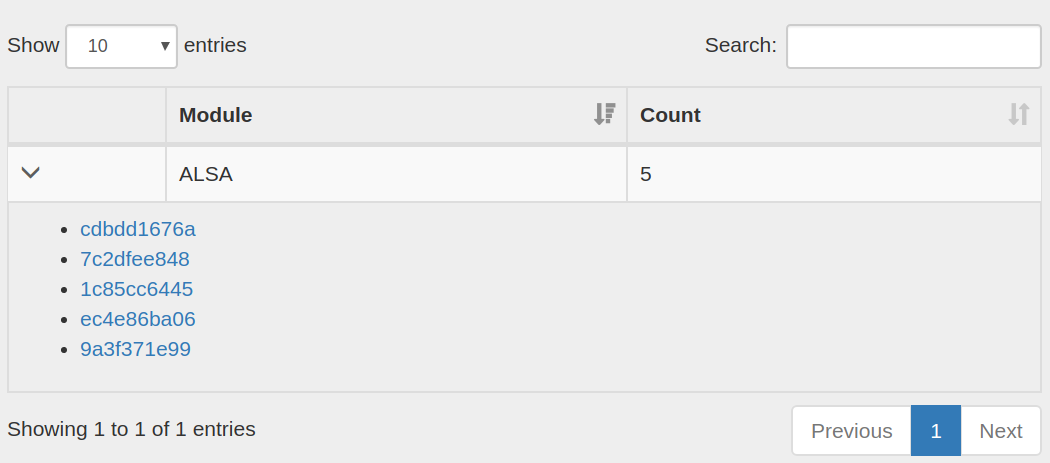
\includegraphics[width=0.9\linewidth]{Figures/Linvis/linvis_modules.png}
  \caption{Table showing the modules involved in a merge, listing the
    commits that modify this module.}
  \label{fig:linvis_modules_results}
\end{figure}

The authorship tab is similar to the files tab, but shows the authorship
information. It shows the sum of the lines added, removed, modified, and
the delta within the \mt{}. It also shows the number of files that were
modified by the author. The details are organized slightly differently
than in the files tab. Instead of showing the commits that make the
modifications, \tool{} shows the individual files that are modified, as
well as the commit hash. As multiple files can be modified in the same
commit, commit hashes are not unique in this table. The authors tab is
shown in Figure~\ref{fig:linvis_authors_results}.

\begin{figure}[htpb]
  \centering
  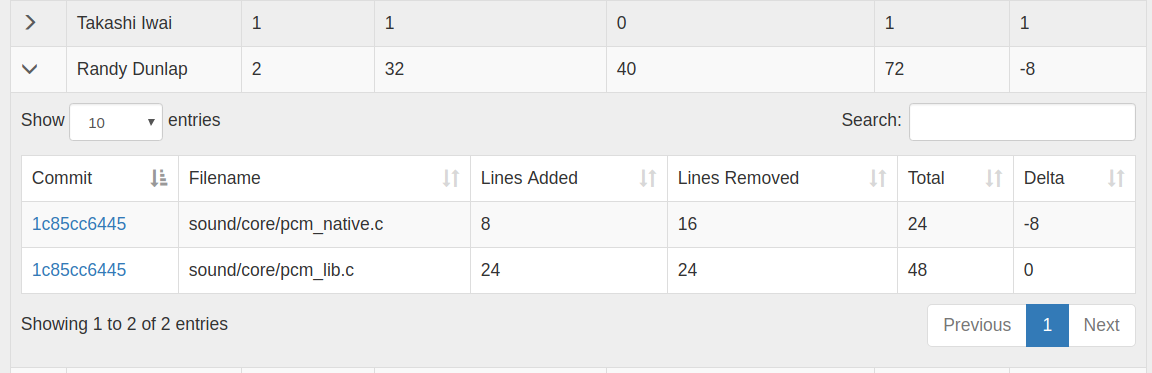
\includegraphics[width=0.9\linewidth]{Figures/Linvis/linvis_authors.png}
  \caption{Table showing the authors who made changes in a merge. The
    entry for Randy Dunlap is expanded, showing the files that Randy
    modified in this merge.}
  \label{fig:linvis_authors_results}
\end{figure}

\section{Visualization}\label{sec:visualization}

While the summarizations are potentially useful, the visualizations are
what make \tool{} different from the other tools that are visualizing
the DAG\@. \tool{} provides access to three visualizations, each with a
specific intention.

\subsection{List Tree}\label{sub:list_tree}

\begin{figure}[htpb]
  \centering
  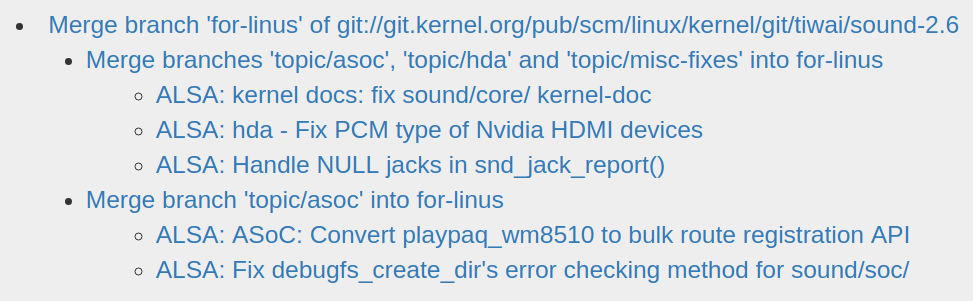
\includegraphics[width=0.9\linewidth]{Figures/Linvis/linvis_list_tree.png}
  \caption{The List Tree Visualization}
  \label{fig:linvis_list_tree}
\end{figure}

The list tree, depicted in Figure~\ref{fig:linvis_list_tree}, is
constructed from nested lists. The indentation level indicates the
hierarchy of the tree. This visualization is text-based, making
searching simple through the browser text search functionality. The top
item in the list is the root of the tree; item node will be indented
further than this item. Due to the complexity of some of the trees, this
tree visualization is rooted at the node that is currently selected.
\tool{} also provides breadcrumbs showing the path that the current
repository event took to being merged into the root of the \mt{} to
ensure that a user can navigate both toward the root and toward the
leaves using this visualization.

\subsection{\rt{} Tree}
\label{sub:rt_tree}

\begin{figure}[htpb]
  \centering
  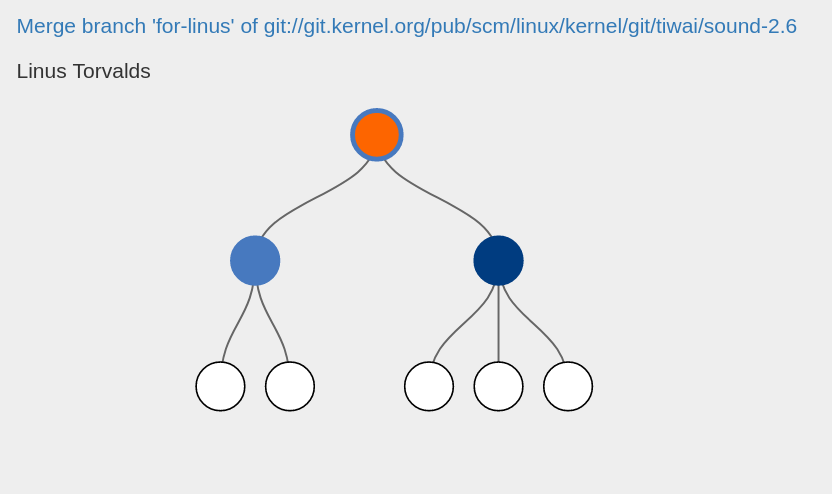
\includegraphics[width=0.9\linewidth]{Figures/Linvis/linvis_reingold_tree.png}
  \caption{The \rt{} tree visualization with the root currently
    selected. The root is at the top, the leaves are depicted as the
    white circles with no children.}
  \label{fig:linvis_reingold_tree}
\end{figure}

The \rt{} tree~\cite{Reingold1981} visualization, depicted in
Figure~\ref{fig:linvis_reingold_tree}, is the classic tree
visualization. The root is at the top, leaves are at the bottom, and the
edges between the nodes showing the parent-child relationship.

The \rt{} tree was designed with the goal of producing trees that looked
tidy. Proposed by Wetherell and Shannon\cite{Wetherell1979}, there were
three aesthetic requirements behind the design of tidy trees;

\begin{itemize}
  \item

    Nodes at the same depth in the tree must be aligned, and each level
    should be parallel.

  \item

    The left and right children must be positioned to the left and right
    of their parent.

  \item

    The parent should be centered above the two children.

\end{itemize}

These requirements are necessary, but not sufficient for producing
visually appealing trees. Reingold and Tilford propose an additional
aesthetic requirement; subtrees should be drawn identically regardless
of position in the tree, and that the reflection of the tree should
produce a mirror-image of the original tree. The entire goal is to
produce trees that are aesthetically pleasing and easily understandable.

In our visual metaphor, the white nodes indicate a commit, while the
colored nodes indicate merges. The merges are colored in shades of blue
to indicate the number of children of that node. Darker shades of blue
indicate more nodes, while lighter shades indicate fewer nodes. The
repository event that is currently being inspected will be filled with
pumpkin orange, but the outline will remain the original color.
Initially, the node representing the current repository event will be
centered in the window, and the title and author of the node are
presented above the visualization. Clicking on a node will center that
node and update title and author. The title is hyper-linked to the page
for that commit, clicking on the title will navigate to the node that
was selected. Clicking and dragging will move the tree in the view,
scrolling will zoom the tree.

\subsection{Pack Tree}
\label{sub:pack_tree}

The Pack Tree\cite{Wang2006} is used for quickly displaying an overview
of large hierarchical data. The original use-case was the file system,
where there are usually many files, but few levels of directories,
creating a very wide but shallow tree. This metaphor is directly
comparable with the structure of a git repository. The commits are
files, they contain the information, rather than being structural. The
merges map to the directories, structurally grouping the commits in a
logical fashion.

\begin{figure}[htpb]
  \centering
  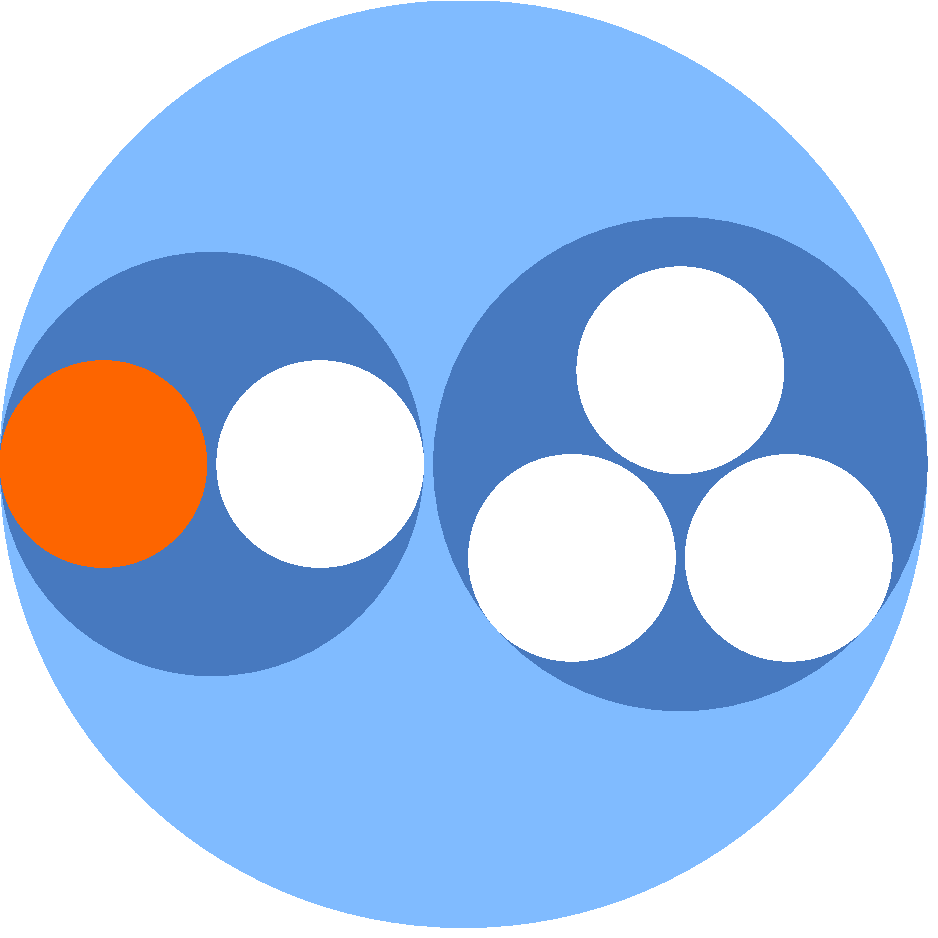
\includegraphics[width=0.4\linewidth]{Figures/Linvis/linvis_bubble.pdf}
  \caption{The pack tree visualization; the root depicted as the
    outer-most circle, containing all other nodes, the leaves depicted
    as white circles containing no other nodes. The currently selected
    node shown in pumpkin orange.}
  \label{fig:linvis_bubble_tree}
\end{figure}

Our goal in providing this visualization is to quickly show the topology
of the merge. With the \rt{} tree, it can be difficult to understand
just how big the large \mt{} are, as they don't fit on the screen. The
Pack Tree uses a set theory-like model for describing the hierarchical
structure. Mapping the pack tree metaphor with the tree, leaves are the
smallest nodes, containing no other nodes; inner nodes contain other
nodes within them; the root is the outermost circle, containing all
other nodes within it.

The bubble tree\cite{Boardman2000} was seen as a possible visualization
for the trees, as it uses a similar metaphor but due to limitations with
the bubble tree, the pack tree seemed more suitable with our goals. The
initial bubble tree visualization starts with a single circle, the root.
Hovering over that circle shows the contents of the node. This works
recursively, hovering the cursor over an inner node will reveal the
contents of that node. While this is designed to prevent overwhelming
users, the user cannot quickly determine what the tree looks like
without hovering their cursor over each inner node. Due to this
limitation, the pack tree was a better option.

An example of the pack tree visualization used in \tool{} is depicted in
Figure~\ref{fig:linvis_bubble_tree}. The outer-most circle that contains
the other circles is the root node. Nodes that are not leaves are
colored in a shade of blue. Darker blue indicates that the node is
deeper in the tree; the root is shaded with the lightest blue. The
commits are colored white. The node that represents the repository event
that is currently being inspected will be shown in pumpkin orange.
